%---------------------------------------------------------------------
%   documentclass
%---------------------------------------------------------------------
\documentclass[a4paper]{article}

%---------------------------------------------------------------------
%   packages
%---------------------------------------------------------------------
\usepackage{mathtools}
\usepackage[english]{babel}
\usepackage[enc=cp1250]{hrlatex}
\usepackage[T1]{fontenc} %nice font
\usepackage{lmodern} %smooth font
\usepackage{hyperref}
\usepackage{amsmath}
\usepackage{amsthm}
\usepackage{cite} %bibtex
\usepackage{enumitem}
\usepackage[pdftex]{graphicx} %for \includegraphics command
\usepackage{titlesec} %section titles font size change
\usepackage{color} %for \definecolor
\usepackage{colortbl} %for \rowcolor command
\usepackage{wrapfig} %for wrapfigure
\usepackage{tikz}
\usepackage{multirow}
\usepackage{floatflt} %to have tables and text beside
\usepackage{scalefnt}

%---------------------------------------------------------------------
%   margins
%---------------------------------------------------------------------
\oddsidemargin 0.0in
\evensidemargin 0.0in
\textwidth 6.1in
\textheight 23.94cm
\topmargin -0.35in

%---------------------------------------------------------------------
%   various settings
%---------------------------------------------------------------------
\pgfrealjobname{dottg} % <-- NOTE: this needs to be the real document's basename
                        %     (else you'll only get an empty output file)

\newif\iffinal % introduce a switch for draft vs. final document
\finaltrue % use this to compile the final document
\iffinal
  \newcommand{\inputTikZ}[1]{%
    \input{#1.tikz}%
  }
\else
  \newcommand{\inputTikZ}[1]{%
    \beginpgfgraphicnamed{#1-external}%
    \input{#1.tikz}%
    \endpgfgraphicnamed%
  }
\fi

\setlist{nolistsep} %so that lists have normal spacing

\renewcommand\baselinestretch{1.3} %line-spacing

\graphicspath{{./pics/}} %picture dir

\titleformat{\section}{\LARGE\bfseries}{\thesection}{1em}{} %section titles
\titleformat{\subsection}{\large\bfseries}{\thesubsection}{1em}{} %subsection titles

\definecolor{tablehead}{RGB}{238,233,233} %nice smooth grey

%---------------------------------------------------------------------
%   environments
%---------------------------------------------------------------------
\renewenvironment{abstract}[1]
{
    \noindent
	\Large
	\begin{center}
		\textbf{#1}
	\end{center}
	
	\normalsize
	
	\addtolength{\leftskip}{1in}
	\addtolength{\rightskip}{1in}
	\setlength{\parindent}{0in}
}
{
}

\newenvironment{itemizesp}
{
    \begin{itemize}
}
{
    \end{itemize}
}

\newtheorem{definition}{Definition}
\newtheorem{theorem}{Theorem}

%---------------------------------------------------------------------
%   magic code
%---------------------------------------------------------------------
% Here it is: the code that adjusts justification and spacing around caption.
\makeatletter
% http://www.texnik.de/floats/caption.phtml
% This does spacing around caption.
\setlength{\abovecaptionskip}{6pt}   % 0.5cm as an example
\setlength{\belowcaptionskip}{6pt}   % 0.5cm as an example
% This does justification (left) of caption.
\long\def\@makecaption#1#2{%
  \vskip\abovecaptionskip
  \sbox\@tempboxa{#1: #2}%
  \ifdim \wd\@tempboxa >\hsize
    #1: #2\par
  \else
    \global \@minipagefalse
    \hb@xt@\hsize{\box\@tempboxa\hfil}%
  \fi
  \vskip\belowcaptionskip}
\makeatother

%---------------------------------------------------------------------
%   document
%---------------------------------------------------------------------
\begin{document}
%---------------------------------------------------------------------
%   FRONTMATTER ------------------------------------------------------
%---------------------------------------------------------------------
    %\frontmatter
    \setlength{\parindent}{0pt}
    \pagestyle{empty}
%    \setcounter{page}{200} %TODO_FINAL - change in final
    \noindent

    %---------------------------------------------------------------------
    %   title page
    %---------------------------------------------------------------------
    \begin{center}
        \begin{minipage}{0.30\textwidth} 
\includegraphics[width=38mm]{logouk.png} \end{minipage}
        \begin{minipage}{0.69\textwidth}
        \textbf{\large\sc
            Department of Computer Science, \\
            Faculty of Mathematics, Physics and Informatics in Bratislava, \\
            Comenius University
        }
        \end{minipage}

        \vskip 5cm

        \begin{center} \line(1,0){250} \end{center}
        {\LARGE\sc Distance oracles for timetable graphs } \\
        \large{(Master thesis)}
        \vskip 0.5cm
        \textbf{\large Franti�ek Hajnovi�}
        \begin{center} \line(1,0){250} \end{center}

        \vfill
    \end{center}

    \textbf{Program}: Informatics 9.2.1 \\
    \textbf{Advisor}: doc. RNDr. Rastislav Kr�lovi�, PhD.   \hfill Bratislava 2012

    \pagebreak

    %---------------------------------------------------------------------
    %   empty page
    %---------------------------------------------------------------------
    \pagebreak

    %---------------------------------------------------------------------
    %   declaration of honesty
    %---------------------------------------------------------------------
    {~}\vfill

    I hereby declare that I wrote this thesis by myself, only with the help of the referenced literature, under the careful supervision of my thesis advisor.
    \vskip 1cm
    \hfill ............................

    \pagebreak

    %---------------------------------------------------------------------
    %   acknowledgements
    %---------------------------------------------------------------------
    \section*{Acknowledgements}
    I would like to thank ...

    \pagebreak

    %---------------------------------------------------------------------
    %   abstract
    %---------------------------------------------------------------------
    \begin{abstract}{Abstract}
        This thesis deals with the shortest path queries on timetable graphs - i.e. graphs that represent timetables (of e.g. Slovak bus network). Firstly we investigate, if some properties (such as low highway dimension) are propagated (and to what extent) from the underlying graph to the timetable graph. Based on these facts, we show how to compute reasonably fast an accurate distance oracle on timetable graphs, that would efficiently answer shortest path queries, thus finding quick timetable connections between any pair of nodes. \\

		Key words: \textbf{distance oracles}, \textbf{timetable graphs}, \textbf{timetable}, \textbf{highway dimension}
	\end{abstract}	

    \begin{abstract}{Abstrakt}
        V tejto pr�ci...\\

		Kl��ov� slov�: \textbf{distance oracles}, \textbf{timetable graphs}, \textbf{timetable}, \textbf{highway dimension}
	\end{abstract}	
	
    \pagebreak

    %---------------------------------------------------------------------
    %   contents
    %---------------------------------------------------------------------

    \tableofcontents

    \pagebreak

%---------------------------------------------------------------------
%   MAINMATTER  ------------------------------------------------------
%---------------------------------------------------------------------
    %\mainmatter
    \pagestyle{plain}
    \setcounter{page}{1}
    \setlength{\parindent}{40pt}

    %---------------------------------------------------------------------
    %   introduction
    %---------------------------------------------------------------------
    %\input parts/introduction.tex

    \section{Introduction}
    World is getting smaller every day, as new technologies constantly make communication and traveling faster and more effective then yesterday. Road network, Internet and many other networks are becoming more evolved and denser which also brings along new problems. In order to fully take advantage of such huge networks, we must have efficient algorithms that operate on these networks and give us answers to many questions. Among many others, one that we take particular interest in is the question: ``What is the shortest path from place $x$ to place $y$''?

    %TODO - obrazok najkratsia cesta

    \begin{floatingtable}{
        \small
        \begin{tabular}{c|c|c|c}
            %legend
            \hline
                \rowcolor{tablehead}
%                place & h & nh & \\
                \multicolumn{2}{>{\columncolor{tablehead}}c|}{\textbf{Place}} & \multicolumn{2}{>{\columncolor{tablehead}}c}{\textbf{Time}} \\
                \hline
                \rowcolor{tablehead}
                \textbf{From} & \textbf{To} & \textbf{Departure} & \textbf{Arrival} \\
            %data
            \hline
                A & B & 10:00 & 10:45 \\
                A & B & 11:00 & 11:45 \\
                A & B & 12:00 & 12:45 \\
                A & C & 9:30 & 10:00 \\
                A & C & 10:15 & 10:45 \\
                C & D & 11:00 & 11:30 \\
                C & D & 13:00 & 13:30 \\
                C & D & 12:20 & 12:35 \\
                C & D & 12:40 & 12:55 \\
                C & D & 13:00 & 13:15 \\
                C & B & 12:20 & 12:50 \\
                C & B & 13:30 & 14:00 \\
                D & A & 13:00 & 14:00 \\
        \end{tabular}}
        \caption{\label{tab:timetable01} An example of a timetable}
        \normalsize
    \end{floatingtable}

    In different networks, this question can make different sense. In the road network, we would like to obtain a sequence of intersections we have to visit in order to reach our destination, driving the shortest possible time (or the smallest possible distance) . GPS devices and the likes of Google maps have to deal with this problem. In the case of Internet network, we might be interested in the shortest path to a destination computer in terms of router hops. In a network of social acquaintances, the smallest number of persons connecting us with e.g. guitarist Mark Knopfler or Liona Boyd could be expressed as a shortest path problem. Many problems in artificial intelligence (e.g. planning of actions) can be expressed (or include) as a shortest path problem.

    %TODO - obrazok socialna siet

    The importance of finding a shortest path in a graph is also obvious from the amount of algorithms and approaches we have nowadays to tackle this problem. In this thesis, we will focus on a more specific problem - finding a shortest connection from place $x$ at the time $t$ to place $y$, given a timetable of connections between nodes in the graph. This problem can be transformed and reduced to the original shortest path problem, but we may take advantage of the specific structure of the graphs representing timetables and find shortest connections more efficiently. Let us formulate the problem at hand more formally.

    Intuitively - a timetable is just a set of \emph{elementary connections} between pairs of nodes in a graph. Let us therefore introduce the definition of a timetable.\\

    \begin{definition}
        \textbf{Timetable on a graph $G$} \\
        A timetable on a given graph $G$ is a set $T_{G} = \{(x, y, p, q)|(x, y) \in E_{G}, \; p, q \in N, \; p < q \}$. An element of T is called an \textbf{elementary connection} and $x$ [$y$] and $p$ [$q$] are the \textbf{departure [arrival] node} and \textbf{time}. Graph $G$ is the \textbf{underlying graph} of timetable $T$.
    \end{definition}

    \noindent Note: G may be directed or undirected - definition is the same for both. Also, we usually meet with timetables using hours or minutes when specifying time. We can easily convert between such time units and natural numbers, so in what follows, we will freely use time expressed in its classical form instead of natural numbers, as found convenient.

    \begin{figure}[h!]
        \begin{center}
            \inputTikZ{./tikzpics/basegraph}
        \end{center}
        \caption{\label{fig:underlying01} Underlying graph of the timetable in ~\ref{tab:timetable01}}
    \end{figure}

    \begin{definition}
        \textbf{Connection from $x$ to $y$ in a given timetable $T_{G}$} \\
        A connection from $x$ to $y$ in a given timetable $T_{G}$ is a sequence of \emph{elementary connections} $e_{1}, e_{2}, ..., e_{k}, \; k \geq 1, \; e_{i} = (x_{i}, y_{i}, p_{i}, q_{i})$, such that $x_{0} = x$, $x_{k} = y$ and $\forall i \in \{2, ..., k\}: (x_{i} = y_{i - 1}, \; p_{i} \geq q_{i - 1})$. \\
        \noindent Connection \textbf{starts} at the \emph{departure time} $p_{1}$. \\
        \noindent \textbf{Size (length)} of the connection is $q_{k} - p_{1}$.
    \end{definition}

    %TODO - transitive closure

    \begin{definition}
        \textbf{Shortest timetable connection (STC) problem} \\
        Given a graph $G$, two of its vertices $x \neq y$, integer $t \in N$ and a timetable on the graph $T_{G}$, what is the shortest \emph{connection} from $x$ to $y$ that \emph{starts} at a \emph{time} $s \geq t$.
    \end{definition}

    %TODO - obrazok timetable graph

        \subsection{Applications}
        We have already mentioned a few applications of the algorithm looking for shortest path in a graph. Many interesting examples can be found in the Christian Sommer's PhD thesis~\cite{sommerthesis10}. As for finding the shortest timetable connection, following applications serve as a motivation: \\

        \begin{itemizesp}
            \item \textbf{Search engines for (inter)national railways}: These are search engines where one specifies the desired departure station and time and destination station and leaves the job on the engine to find the shortest connection. Often we meet with advanced systems that incorporate train, bus and even airplane timetables all into the same search engine, or offer extra features such as required time for a change, traveling cost restrictions etc...
            \item %todo - dalsie applications
        \end{itemizesp}

        \subsection{Traditional approaches to shortest path problem}
        We will shortly present some of the well known algorithms that solve shortest path problems.

            \subsubsection{Dijkstra's algorithm}
            The most famous of all, Dijkstra's algorithm, was published in 1959 by Edsger Dijkstra. It's original implementation runs in time $\mathcal{O}(n^2)$ (where $n=|V_{G}|$) and finds the shortest path from a given vertex $v$ to every other vertex in a directed graph (if the graph is strongly connected), thus producing a so called \emph{shortest path tree} (that is, a tree rooted at $v$ with every path starting at $v$ being a shortest path in the original graph) . A restriction is posed that edge weights must be positive.

            Briefly sketching the idea, in one iteration the algorithm visits the closest (with respect to the starting point $v$) so far unvisited vertex and updates the estimates of distances to all of its neighbors. The idea is to maintain an invariant, that for a visited node we know the correct shortest distance from $v$ which can be achieved just by moving along already visited vertices \cite{Tea97}.

            Dijkstra's algorithm has been adjusted and tuned many times to achieve higher performance (better time complexity). Currently best bound is provided by an implementation using Fibonacci heap as a priority queue for next-visited-node selection. The resulting time complexity is $\mathcal{O}(m + n\log n)$ (where $m=|E_{G}|$) \cite{sommerthesis10}.

            \subsubsection{Bellman-Ford algorithm}
            Bellman-Ford algorithm considers also the graphs with negative edge weights. It differs from Dijkstra's algorithm mostly in the fact, that it does not apply the greedy next-visited-node selection (which prohibits the negative edge weights), but instead \emph{relaxes} each edge $n - 1$ times, hence the time complexity $\mathcal{O}(n m)$. The relaxation itself means checking if the estimate of the distance to the edge's endpoint could be improved with estimate of the edge's start point plus the weight of the edge.

            Because of the negative edge weights, algorithm must also check for negative cycles, which, however, does not increase the overall complexity. Similarly to Dijkstra's algorithm, it produces a shortest path tree rooted at the starting vertex.

            \subsubsection{A* search algorithm}
            A* is an algorithm that uses heuristics to speed up finding of the optimal path from a starting vertex $v$ to the destination vertex $u$. The next visited node is the one that minimizes the (true) distance from $v$ plus the heuristic estimate of distance to $u$. The complexity of the A* algorithm depends on the heuristics. In the worst case, it may have to expand number of vertices exponential in the shortest path length. Only if the heuristics $h$ provides a very good estimate \footnote{By good estimate, we mean $|h(x) - h*(x)| = \mathcal{O}(log*(x))$ where $h*(x)$ is the optimal heuristics (true distance)}, the number of expanded vertices is polynomial in the size of the shortest path \cite{zuiprednaska}. Unfortunately, computing the heuristics itself in that case may require too much time and thus considerably increase the time complexity of the algorithm.

            %TODO - check the performance of A* on road networks...

            \subsubsection{Floyd-Warshall algorithm}
            From the category of dynamic programming, Floyd-Warshall algorithm computes shortest paths between all pairs of vertices in $\mathcal{O}(n^{3})$.

        \subsection{Problem with traditional approaches}
        With the arsenal of algorithms (from which we have mentioned just a few), one may wonder about our contribution to the STC problem, which may, as we have stated, be reduced to finding shortest path in a specific graph. That is, of course, a possible approach - the mentioned algorithms are polynomial, almost linear in time complexity. However, consider a road network of Europe, which may contain %TODO - find out!!
        tens of millions of intersections and even several times more road segments (connections between two intersections) . If an online server hosting interactive map (like Google Maps) run Dijkstra's algorithm on such a large scale network for every query, it would not be able to answer those queries in real time, as required by users.

        Other straightforward approach would precompute every shortest path and then answer shortest path queries in a constant time. That would, however, require a large table of size $\mathcal{O}(n^3)$ \footnote{For every pair of vertices, we would store the shortest path}, or at least $\mathcal{O}(n^2)$ \footnote{We store just the last vertex on the way to the destination, but the query then takes $\mathcal{O}(n)$ in the worst case}. In any case, the construction itself (not to mention the required memory) is very costly - with Floyd-Warshall algorithm and the mentioned scale, the computation might take more than $(10^{7})^{3} = 10^{21}$ steps.

        We have yet to mention timetables in the previous discussion. In the case of the graph representing a given timetable \emph{on a graph of the size of the European road network} (in the section~\ref{sec:preliminaries}, %TODO - exact subsection
        there are descriptions how to construct timetable graphs), we obtain even bigger input for the shortest path problem. Later in the Preliminaries section, we will give more details about these graphs.

        \subsection{Shortest paths via distance oracles}
        Due to the limitations described above, many other approaches were explored. The term \emph{Distance oracle} (DO) was first coined in 2001 by Thorup and Zwick~\cite{apxdo05} (for a definition, see section~\ref{sec:preliminaries}) %TODO - exact subsection
        . The DO based method for shortest path retrieval consists of a preprocessing of the graph to a structure (the distance oracle), which then answers (not necessarily correctly) queries for shortest path, using as little computation as possible.

        Essentially, the DO method may be characterized by four parameters, all of which we try to minimize, but among which we have to make compromises:

        \begin{enumerate}
            \item preprocessing time
            \item size of the resulting structure
            \item query time
            \item \emph{stretch} - worst case ratio agains optimal path size
        \end{enumerate}
        \hspace*{\fill}

        \noindent The approaches we have mentioned are the extreme cases, where some parameters are completely minimized while others are too large.

        \subsection{Organization of this paper}
        This thesis is organized in following sections:

        \begin{enumerate}
            \item \textbf{Preliminaries}: we formulate necessary definitions and timetable graph constructions used throughout the rest of the thesis
            \item \textbf{Related work}: main results in the area of distance oracles, shortest path queries and distance labelling, useful in the following sections
            \item \textbf{Properties propagation upon time-expansion}: we show how (and to what extent) certain properties of the graph are preserved when time-expanded to a timetable graph
            \item \textbf{Proposed distance oracles for timetable graphs}: we present our approach to solve STC problem, based on distance oracles
            \item \textbf{Implementation and results}: we present our implementation and obtained results of the algorithm's behavior in practice
            \item \textbf{Conclusion}: we conclude
        \end{enumerate}
        \hspace*{\fill}

        \noindent Each section may contain several sub-sections and further sub-sub-sections. For words in \emph{italic}, there is a definition provided in this thesis.

    \pagebreak

    %---------------------------------------------------------------------
    %   preliminaries
    %---------------------------------------------------------------------
    %\input parts/preliminaries.tex

    \section{Preliminaries}
    \label{sec:preliminaries}
    In this section, we would like to introduce terminology and definitions used later on in the thesis.

    We assume the reader to be familiar with some standard notions from graph theory such as \emph{graph}, \emph{subgraph}, \emph{path}... Much of the terminology we will use can be found in \cite{sommerthesis10}. We will provide only the definitions of not well established terminology and our own definitions.

    If not stated otherwise, by a graph we will mean a directed graph (\emph{digraph}) with non-negative edge (\emph{arc}) weights.

        \subsection{Common definitions}
        \begin{definition}
            \textbf{Distance between nodes $x$ and $y$ in graph $G$} \\
            Denoted $d_{G}(x, y)$, distance between $x$ and $y$ in $G$ is the length of the shortest path from $x$ to $y$: \\
            $\displaystyle d_{G}(x, y) = \min_{\substack{P \in \mathcal{P}(x, y)}} l(P)$
            where $l(P)$ is the length of the path $P$ and $\mathcal{P}(x, y)$ is the set of all paths from $x$ to $y$ in $G$.
        \end{definition}

        \begin{definition}
            \textbf{{\boldmath $(prepro_{M}, size_{M}, qtime_{M}, stretch_{M})$} Distance oracle for a graphs $G$} \\
            A $(prepro_{M}, size_{M}, qtime_{M}, stretch_{M})$ distance oracle $M$ for a graph $G$ is a data structure characterized by following properties:
            \begin{enumerate}
                \item $M$ could be created in a \textbf{preprocessing time} $prepro_{M}$ from graph $G$
                \item $M$ takes up $size_{M}$ bits of memory (\textbf{DO size})
                \item $M$ answers queries for shortest path between pair of vertices in $G$ in maximum time of $qtime_{M}$ (\textbf{query time} of DO)
                \item the answer provided by $M$ is not worse than $stretch_{M}$ times the optimum value (\textbf{stretch} of DO)
            \end{enumerate}
        \end{definition}

        %TODO - SVG
        \begin{figure}[h!]
            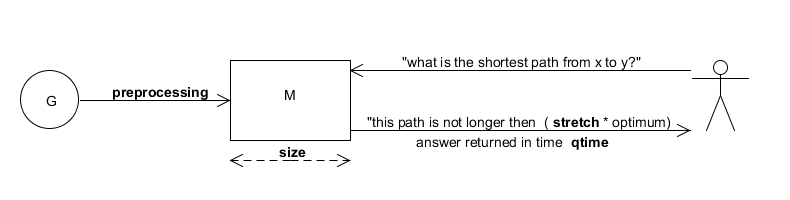
\includegraphics[scale=0.57]{dodiagram.png}
            \caption{\label{fig:dodiagram} Diagram showing the properties of a distance oracle}
        \end{figure}

        \begin{definition}
            \textbf{{\boldmath $(prepro_{F}(G), size_{F}(G), qtime_{F}(G), stretch_{F}(G))$} Distance oracle method for a class of graphs $\mathcal{G}$}\\
            Let $prepro_{F}(G)$, $size_{F}(G)$ and $qtime_{F}(G)$ be functions from $\mathcal{G}$ to $N$ and $stretch_{F}(G)$ a function from $\mathcal{G}$ to $R$. A $(prepro_{F}(G), size_{F}(G), qtime_{F}(G), stretch_{F}(G))$ distance oracle method $F$ for a class of graphs $\mathcal{G}$ is an algorithm, that for each graph $G' \in \mathcal{G}$ produces a $(prepro_{F}(G')$, $size_{F}(G')$, $qtime_{F}(G')$, $stretch_{F}(G'))$ \emph{distance oracle}. \\
            \noindent We will refer to the four functions of the DO method as \textbf{preprocessing time}, \textbf{DO size}, \textbf{query time} and \textbf{stretch} respectively.
        \end{definition}

        \noindent Note 1: alternatively, we may write $(\mathcal{O}(f(n)), \mathcal{O}(g(n)) ...)$ \emph{DO method}, meaning that $\exists prepro_{F}(G) = \mathcal{O}(f(n))$ and $\exists size_{F}(G) = \mathcal{O}(g(n))$ ... such that we have corresponding DO method. \\

        \noindent Note 2: in \cite{apxdo05}, no proper definition of a distance oracle was made. %TODO - what did they mean by DO then?
        In \cite{sommerthesis10} a term DO means both - an algorithm together with the data structure it produces. We saw fit to split the definition and refer to the structure itself as a distance oracle, and to the algorithm as a distance oracle method.

        \subsection{Classes of graphs}
        \begin{definition}
            \textbf{Power-law graphs} \cite{powerlaw09} \\
            Power-law graphs is a class of graphs, in which a number of nodes with degree $x$ is proportional to $x^{\tau}$, for a constant $\tau \in (2, 3)$.
        \end{definition}
        %TODO - make more accurate with scale-free etc... from Sommmer

        \noindent We also meet with term \textbf{scale-free network} or \textbf{small world}.

        \noindent Many real-world networks have power-law structure, or at least are though to have. One such example is airline network, which nicely demonstrate the definition of a power-law graph. There are several (not many) huge airports, that are linked together accross the world. Apart from these links, they have plenty of other connections to other, smaller airports, possibly within continent or surrounding countries. The smaller airports do not have many connections but on the other hand are more ubiquitous. Overall, we can usually get from one airport to any other one following a short chain of flights, thus the notion of a \emph{small world.}

        \subsection{Graph properties}
            \subsubsection{Highway dimension}
            \begin{definition}
                \textbf{Highway dimension for an undirected graph $G$} ~\cite{highwaydim10} \\
                Highway dimension (HD) for an undirected, edge-weighted graph $G$ is the smallest integer $h$, such that
                \vskip 10pt
                \indent $\forall r \in R^{+}, \forall u \in V_{G}, \exists S \subseteq B_{u, 4r}, |S| \leq h,$ such that $\forall v, w \in B_{u, 4r}:$ \\
                \indent \indent if $|P(v, w)| > r$ and $P(v, w) \subseteq B_{u, 4r}$ then $P(v, w) \cap S \neq \emptyset$
                \vskip 10pt
                \noindent where $B_{u, r} = \{v \in G | d(u, v) \leq r\}$ and is called \textbf{ball} of radius $r$ centered at $u$.
            \end{definition}

            \noindent Intuitively, a graph has a low HD, if for any $r$ we have a \emph{sparse} set of vertices $S_{r}$, such that every shortest path longer then $r$ includes a vertex from $S_{r}$. By the set being sparse, we mean that every ball of radius $\mathcal{O}(r)$ contains just a few elements of $S_{r}$.

            \begin{figure}[h!]
                \begin{center}
                    \inputTikZ{./tikzpics/highwaydim}
                \end{center}
                \caption{\label{fig:highdemonstr} Demonstration of a definition of HD. We chose some $r$ ($r = 3$) and some vertex $v$ ($v = C$) to root the ball $B_{v, 4r}$. All the shortest paths \emph{longer} than $r$ \emph{inside} the ball have to contain a vertex from $S$ (orange vertices $C$ and $A$ in our case). The upper bound on $|S|$, considering any ball with any radius, is the required highway dimension. Note: in our case, we had to choose also $A$ to set $S$, since a shortest path from $B$ to $D$ does not include $C$.}
            \end{figure}

            The definition is for undirected graphs. A similar definition can be obtained for directed graphs, using \emph{shortest path covers}. %TODO - why not sufficient to take directed ball

            \begin{definition}
                \textbf{($r$, $k$) Shortest path cover (($r$, $k$)-SPC)} ~\cite{highwaydim10} \\
                A set $C$ is a ($r$, $k$)-SPC of $G$ if and only if $\forall u \in V_{G}, |C \cap B_{u, 2r}| \leq k$ and for every shortest path $P: r < |P| \leq 2r, P \cap C \neq \emptyset$.
            \end{definition}

            \noindent Depending on if the graph is directed/undirected, we choose \emph{directed/undirected ball} in the above definition.
            \begin{definition}
                \textbf{Directed ball} \\
                A \textbf{directed ball} $B_{u, r} = \{v \in G | d(u, v) \leq r \; or \; d(v, u) \leq r\}$
            \end{definition}
            %todo obrazok

            \begin{definition}
                \textbf{Highway dimension for an directed graph $G$} ~\cite{highwaydim10} \\
                Highway dimension (HD) for an directed, edge-weighted graph $G$ is the smallest integer $h$, such that $\forall r \exists (r, h)-SPC$.
            \end{definition}

            \noindent Note: in the above definition, we use shortest path covers with directed balls.

            \begin{definition}
                \textbf{$r(n)$ separator}
            \end{definition}

        \subsection{Timetable graphs}
        In this subsection, we will discuss the construction of a timetable graph out of the given timetable. Terminology \emph{time-expanded} and \emph{time-dependent} graph was inspired by \cite{timetablemodelsalgs07}. %TODO - only inspired?

        \begin{definition}
            \textbf{Time-expanded graph} \\
            Let $T$ be a timetable on $G$. Time-expanded graph from $T$ is an oriented graph $G_{T}$ whose vertices are pairs $[v, t], v \in G$ and $\exists (x, y, p, q) \in T$ such that $p = t$ or $q = t$. Edges of $G_{T}$ are formed by
            \begin{enumerate}
                \item $([x, p], [y, q]), ;\ \forall (x, y, p, q) \in T$
                \item $([x, p], [x, q]), [x, p], [x, q] \in V_{G_{T}}, p < q$ and $\not \exists [x, r] \in V_{G_{T}}: p < r < q$.
            \end{enumerate}
            Weight $w$ of any edge $((x, p), (y, q))$ in $E_{G_{T}}$ is $w((x, p), (y, q)) = q - p$.
        \end{definition}

        \noindent Intuitively, nodes in the time-expanded graph correspond to events - when a connection arrives or departs from a given place. Edges are then \emph{elementary connections} and a waiting at a given place.

        \begin{figure}[h!]
            \scriptsize
            \begin{center}
                \inputTikZ{./tikzpics/timeexpanded}
            \end{center}
            \caption{\label{fig:timeexp01} Time-expanded graph from the timetable in ~\ref{tab:timetable01}}
        \end{figure}

        If we wanted to use algorithms for shortest path to find the optimal connection, we would need a little further modification, where for every $x \in V_{G}$ ($G$ being the underlying graph), we add a new vertex $x_{dest}$ to $G_{T}$ and edges $([x, p], x_{dest}), ;\ \forall [x, p] \in V_{G_{T}}$ with zero weight (see figure ~\ref{fig:shpathtimeexp}). We can then ask about shortest path from $[x, t]$ to $y$ that would correspond to looking for optimal connection from $x$ to $y$ at a time $t$.

        \begin{figure}[h!]
            \scriptsize
            \begin{center}
                \inputTikZ{./tikzpics/timeexpanded_search}
            \end{center}
            \caption{\label{fig:shpathtimeexp} A portion of the time-expanded graph from the timetable in ~\ref{tab:timetable01}, modified (green edges and vertices) to enable finding optimal connections via shortest path queries}
        \end{figure}

        Sometimes it will be more convenient, if all the events were happening at times being multiple of some value.

        \begin{definition}
            \textbf{Approximate time-expanded graph} \\ %to moje
            Let $T$ be a timetable on $G$ and $k \in N$. Approximate time-expanded graph from $T$ is an oriented graph $G_{T, k}$ whose vertices are $[v, t], v \in G, t = k \cdot l, l \in N$. Edges of $G_{T, k}$ are formed by
            \begin{enumerate}
                \item $([x, p'], [y, q']), ;\ \forall (x, y, p, q) \in T$ where $p' = \lfloor \frac{p}{k} \rfloor \cdot k$ and $q' = \lceil \frac{q}{k} \rceil \cdot k$
                \item $([x, p], [x, q]), [x, p], [x, q] \in V_{G_{T}}, p < q$ and $\not \exists [x, r] \in V_{G_{T}}: p < r < q$.
            \end{enumerate}
            Edge weights are defined as with \emph{time-expanded graphs}.

            \noindent We will call $k$ a \textbf{granularity} of the approximate time-expanded graph.
        \end{definition}

        \noindent It is possible that we lose some information in the approximate time-expanded graph. %TODO - obrazok
        We will analyze this later on, to show how much information could be lost based on a given \emph{granularity} and how to fix this. %TODO - analyze

        %TODO - discussion about the size
        Consider the London Underground system. It serves 270 stations with 11 lines with a high operating frequency (about 10 minutes on average) and serving above 30 stations on average (note that more lines might serve the same station) ~\cite{LondonUnd}. Therefore, we expect an event to occurs at a given station every $10 \cdot (\frac{270}{11 * 30}) \approx 8$ minutes. If we took a timetable of the underground for one day and made a time-expanded graph from it, how many nodes would it have? London Underground operates about 20 hours a day, which is 1200 minutes. The 8 minute event interval yields about 150 events per station per day. Thus, overall, we have a time-expanded graph with 34500 vertices.

        An approximate time-expanded graph with \emph{granularity} $k = 1$ would, in this case, have $270 \cdot 20 \cdot 60 = 324000$ vertices.

        Both graphs are possible to construct in a linear time with respect to their sizes. They can then serve (with slight adjustment as in ~\ref{fig:shpathtimeexp}) for throughout the day to look for shortest connections using e.g. Dijkstra's algorithm, answering queries relatively quickly.

        However, this was an example of just a small network with 270 nodes in the \emph{underlying graph} of the timetable. The numbers (of nodes in the expanded graphs) we obtain suggest, that such an approach would indeed fail for timetables on a large-scale graphs, as e.g. those for Europe-wide railway system.

        Let us introduce another type of a timetable graph, that is more compact but does not provide all the timetable information.

        \begin{definition}
            \textbf{Time-dependent graph} ~\cite{timetablemodelsalgs07} \\
            Let $T$ be a timetable on $G$. Time-dependent graph from $T$ is a non-weighted oriented graph $\widetilde{G_{T}}$ whose vertex set $V_{\widetilde{G_{T}}} = V_{G}$ and there is an edge between $x$ and $y$ if $\exists (x, y, p, q) \in T$.
        \end{definition}

        \noindent As specified in ~\cite{timetablemodelsalgs07}, ``The lengths of the edges are assigned ``on-the-fly'': the length of an edge depends on the time, in which it will be used in the algorithm...''. Hence the name \emph{time-dependent graph}. This type of graph will not be used much in this thesis, and by \textbf{timetable graph}, we will generally refer to the \emph{time-expanded graph} from a given timetable.


    %classes of graphs
    %   power law, scale free, small-world

    %shortest path problem settings
    %   APSP...

    %properties
    %   hd
    %       obrazok
    %   separator
    %       obrazok


    %timetable graphs - approaches
    %   underlying graph (base)
    %       obrazok
    %   time-expanded graph
    %       obrazok

    \pagebreak

    %---------------------------------------------------------------------
    %   related work
    %---------------------------------------------------------------------
    %\input parts/relatedwrk.tex

    \section{Related work}
    Much of the work done in the area of distance oracles and shortest path queries can be found in a summary~\cite{hajnresearch12}. Most relevant, with regard to this thesis, are the results in \cite{apxdo05}, \cite{highwaydim10}, \cite{distlabel04}.

    An important result was reached by Thorup and Zwick, when they found a DO method for general graphs, that makes it possible to trade \emph{stretch} for a better \emph{preprocessing time} and \emph{DO size}.

    \begin{theorem}
        \textbf{(Thorup and Zwick)} \\
        For the class of general undirected weighted graphs, there is a $(\mathcal{O}(kmn^{1/k}), \mathcal{O}(kn^{1 + 1/k}), \mathcal{O}(k), 2k - 1)$ DO method.
    \end{theorem}

    %uvodne kecy
    %   vela sa toho spravilo
    %   sumar v mojom clanku

    %Thorup and Zwick

    %distance labelling

    %sommer

    %HD

    \pagebreak

    %---------------------------------------------------------------------
    %   properties propagation upon time-expansion
    %---------------------------------------------------------------------
    %\input parts/properties.tex

    \section{Properties propagation upon time-expansion}
    In this section, we would like to show how certain properties are propagated from the \emph{underlying graph} upon time-expansion. \\

    \noindent Following properties will be considered:

    \begin{itemizesp}
        \item Highway dimension
        \item $r(n)$-separator
        \item graph planarity
    \end{itemizesp}

    \pagebreak

    %---------------------------------------------------------------------
    %   proposed distance oracles for timetable graphs
    %---------------------------------------------------------------------
    %\input parts/proposeddo.tex

    \section{Proposed distance oracles for timetable graphs}

    \pagebreak

    %---------------------------------------------------------------------
    %   implementation and results
    %---------------------------------------------------------------------
    %\input parts/implresults.tex

    \section{Implementation and results}
    Following programs are planned to be developed:

    \begin{itemizesp}
        \item Simple program for creating time-expanded graph out of given timetable (C++)
        \item Simple program for converting a graph defined in XML to a picture in PDF format (C++)
        \item Program with an interface for testing DO methods and making statistics (Java)
        \item Implementation of a proposed DO method for timetable graphs
    \end{itemizesp}

    \pagebreak

    %---------------------------------------------------------------------
    %   conclusion
    %---------------------------------------------------------------------
    %\input parts/conclusion.tex

    \section{Conclusion}

    \pagebreak

%---------------------------------------------------------------------
%   BACKMATTER  ------------------------------------------------------
%---------------------------------------------------------------------
    %\backmatter

    %---------------------------------------------------------------------
    %   bibliography
    %---------------------------------------------------------------------

    \bibliographystyle{is-alpha}
    %compile latex, bibtex, latex, latex
    \bibliography{bibl}{}
\end{document} 